\documentclass[]{article}
\usepackage{lmodern}
\usepackage{amssymb,amsmath}
\usepackage{ifxetex,ifluatex}
\usepackage{fixltx2e} % provides \textsubscript
\ifnum 0\ifxetex 1\fi\ifluatex 1\fi=0 % if pdftex
  \usepackage[T1]{fontenc}
  \usepackage[utf8]{inputenc}
\else % if luatex or xelatex
  \ifxetex
    \usepackage{mathspec}
    \usepackage{xltxtra,xunicode}
  \else
    \usepackage{fontspec}
  \fi
  \defaultfontfeatures{Mapping=tex-text,Scale=MatchLowercase}
  \newcommand{\euro}{€}
\fi
% use upquote if available, for straight quotes in verbatim environments
\IfFileExists{upquote.sty}{\usepackage{upquote}}{}
% use microtype if available
\IfFileExists{microtype.sty}{%
\usepackage{microtype}
\UseMicrotypeSet[protrusion]{basicmath} % disable protrusion for tt fonts
}{}
\ifxetex
  \usepackage[setpagesize=false, % page size defined by xetex
              unicode=false, % unicode breaks when used with xetex
              xetex]{hyperref}
\else
  \usepackage[unicode=true]{hyperref}
\fi
\hypersetup{breaklinks=true,
            bookmarks=true,
            pdfauthor={},
            pdftitle={},
            colorlinks=true,
            citecolor=blue,
            urlcolor=blue,
            linkcolor=magenta,
            pdfborder={0 0 0}}
\urlstyle{same}  % don't use monospace font for urls
\setlength{\parindent}{0pt}
\setlength{\parskip}{6pt plus 2pt minus 1pt}
\setlength{\emergencystretch}{3em}  % prevent overfull lines
\setcounter{secnumdepth}{0}

\date{}

\usepackage{graphicx}
\begin{document}

\section{Tecniche di biologia
molecolare}\label{tecniche-di-biologia-molecolare}

\subsection{Enzimi di restrizione}\label{enzimi-di-restrizione}

Enzimi che apportano tagli sui filamenti di DNA vengono chiamati
\textbf{nucleasi}, e si distinguono in:

\begin{itemize}
\itemsep1pt\parskip0pt\parsep0pt
\item
  \textbf{endonucleasi}, se tagliano i legami fosfodiesterici interni in
  una molecola di DNA circolare o lineare;
\item
  \textbf{esonucleasi}, se si legano a una delle due estremità libere e
  iniziano a tagliare in maniera processiva verso l'altra estremità.
\end{itemize}

Gli enzimi di restrizione \textbf{(ER)} sono delle endonucleasi che
provocano delle rotture interne a doppio filamento sul DNA in
corrispondenza di particolari sequenze nucleotidiche.

Le endonucleasi di restrizione si legano ad una sequenza specifica di
DNA, detta \emph{``sito di riconoscimento''}, e tagliano entrambi i
filamenti dell'elica.

Gli ER vengono distinti in ER del I, del II e del III tipo. Gli
\textbf{ER del I e del III tipo} portano l'attività di restrizione e
metilazione nella stessa molecola. Filamenti di DNA \emph{non metilati}
possono essere attaccati da questi enzimi, mentre filamenti metilati ne
impediscono l'azione. Questi enzimi riconoscono una specifica sequenza
di nucleotidi, ma tagliano il DNA in posizioni non specifiche a una
certa distanza dalla sequenza riconosciuta. Poichè il sito di taglio non
corrisponde a una specifica coppia di basi, gli enzimi di restrizione
del I tipo non sono quasi mai utilizzati nelle tecnologie del DNA
ricombinante.

Gli \textbf{ER del II tipo} riconoscono anch'essi specifiche sequenze di
nucleotidi, ma tagliano il DNA all'interno di quelle specifiche
sequenze, chiamate \textbf{siti di taglio}.

La sequenza di riconoscimento per la maggioranza degli ER del II tipo è
lunga 4-6 nucleotidi, ma esistono ER chiamati \textbf{rare cutter} che
riconoscono sequenze più lunghe. La frequenza di taglio di un ER è
legata alla lunghezza della sequenza riconosciuta da quello specifico
enzima. Una sequenza si 4 basi significa una probabilità di taglio di
(1/4)\(^4\), cioè 1 volta ogni 256 nucleotidi.

ER isolati da batteri differenti ma che riconoscono e tagliano la stessa
sequenza nucleotidica sono chiamati \textbf{isoschizomeri}.

La maggior parte degli ER riconoscono sequenze sulla doppia elica del
DNA definite \textbf{palindromiche}, ovvero possiedono la stessa
sequenza sui due filamenti letti in direzione 5' \(\rightarrow\) 3' (es.
la sequenza 5'GAATTC3' riconosciuta dall'ER noto come EcoRI).

L'utilizzo degli enzimi di restrizione é molto semplice; la maggior
parte di essi funziona in semplici tamponi tra pH 7 e 8, generalmente a
37°C. Le condizioni di utilizzo sono comunque sempre specificate dai
fornitori. Per definizione \emph{un'unità di un enzima di restrizione è
la quantità di enzima richiesta per digerire completamente 1 \(\mu\)g di
DNA substrato in un'ora}. Tutti gli enzimi, in condizioni non ottimali,
danno l'\textbf{``effetto star''}, che consiste nella capacità
dell'enzima di ``confondersi'' riconoscendo e tagliando sequenze simili,
ma non identiche a quella target. Per evitare l'effetto target é
opportuno attenersi alle condizioni specificate dai fornitori, con
particolare riferimento al glicerolo e alla quantità di enzima, che non
devono essere mai in eccesso.

\subsubsection{Nomenclatura}\label{nomenclatura}

Per assegnare in modo chiaro ed univoco un codice ad un enzima si è
deciso che:

\begin{itemize}
\itemsep1pt\parskip0pt\parsep0pt
\item
  le prime \textbf{3 lettere} sono prese dal nome del batterio di
  origine. La prima lettera dal genere e le altre due dalla specie (es.
  Eco \textbf{E}scherichia \textbf{co}li);
\item
  tipi differenti dello stesso organismo sono indicati da una
  \textbf{quarta lettera} minuscola (es. Hin\textbf{d} Haemophilus
  influenzae sierotipo Rd, Hin\textbf{f} Haemophilus influenzae
  sierotipo Rf);
\item
  segue una lettere maiuscola o numero che identificano un ceppo
  particolare di batterio (Eco\textbf{R} Escherichia coli ceppo RY13);
\item
  un \textbf{numero romano} indica l'ordine di scoperta qualora dallo
  stesso batterio vengano isolati enzimi diversi.
\end{itemize}

\textbf{Esempio}

\textbf{EcoRI}:

\begin{itemize}
\itemsep1pt\parskip0pt\parsep0pt
\item
  \textbf{E} = genere Escherichia;
\item
  \textbf{co} = speie coli;
\item
  \textbf{R} = ceppo RY13;
\item
  \textbf{I} = prima endonucleasi isolata.
\end{itemize}

Sequenza riconosciuta: G/AATTC - CTTAA/G

\textbf{BamHI}:

\begin{itemize}
\itemsep1pt\parskip0pt\parsep0pt
\item
  \textbf{B} = genere Bacillus;
\item
  \textbf{am} = specie amyloliquefaciens G/GATCC;
\item
  \textbf{H} = ceppo H;
\item
  \textbf{I} = prima endonucleasi isolata.
\end{itemize}

Sequenza riconosciuta: G/GATCC - CCTAG/G

Come fa un organismo che produce una endonucleasi a proteggersi
dall'azione dell'enzima prodotto? Tramite un sistema di
\textbf{protezione per modificazione}.

Dopo aver effettuato il taglio, l'ultimo nucleotide (quello rimasto
``scoperto'') viene metilato. La metilazione non altera la normale
struttura del DNA, ma inibisce il taglio.

Il taglio tramite enzimi di restrizine può generare diversi tipi di
estremità.

Esistono ER in graod di tagliare entrambi i filamenti della doppia elica
nello stesso punto, generando delle \textbf{estremità piatte (blunt
end)}; altri ER, invece, operano un taglio obliquo lasciando delle
\textbf{estremità sporgenti}. In questo caso le estremità possono
sporgere al 5' o al 3' e vengono chiamate \textbf{sticky end}. Frammenti
di DNA generati da tagli con ER possono essere legati tra di loro o
inseriti in un vettore di clonaggio in provetta utilizzando l'enzima DNA
ligasi.

\subsection{L'elettroforesi su gel}\label{lelettroforesi-su-gel}

Molecole diverse di DNA, RNA e proteine possono essere separate modiante
elettroforesi su gel perchè differiscono nella loro carica elettrica,
dimensione e struttura.

L'elettroforesi rappresenta lo strumento classico di cui si serve un
biologo molecolare per \emph{separare}, \emph{identificare} e
\emph{isolare} frammenti di DNA o RNA.

Le prime elettroforesi, che venivano eseguite in fase liquida, sono
state soppiantate da quelle in fase solida, più riproducibili. Le
matrici solide generalmente usate sono costituite da:

\begin{itemize}
\itemsep1pt\parskip0pt\parsep0pt
\item
  \textbf{gel di agarosio}, uno zucchero solubile in acqua alla
  temperatura di ebollizione che diventa solido quando si raffredda,
  formando una matrice attraverso dei legami idrogeno tra le catene
  lineari;
\item
  \textbf{gel di poliacrilammide}, si forma tramite copolimerizzazione
  di acrilammide, un monomero solubile in acqua, e di un agente che
  forma legami trasversali così da formare un reticolo tridimensionale.
\end{itemize}

I gel più utilizzati in biologia molecolare sono quelli di agarosio con
percentuali varianti tra 0,7 e 2\%. A basse concentrazioni di agarosio
si risolvono meglio i pesi molecolari alti, mentre ad alte
concentrazioni si risolvono meglio i pesi molecolari bassi. Per
risolvere frammenti di DNA molto piccoli (tra 200 e 1 bp) si ricorre a
gel di poliacrilammide.

I due tipi di gel differiscono per le dimensioni dei pori del reticolo:
gel con pori grandi permettono la separazione di molecole di grandi
dimensioni, gel con pori piccoli separano molecole di dimensioni
limitate.

La separazione tramite elettroforesi consiste nel movimento di una
molecola carica sottoposta ad un campo elettrico. Questo campo elettrico
viene creato dal collegamento di un alimentatore di corrente elettrica
all'apparecchio per l'elettroforesi.

Poiché gli acidi nucleici sono molecole cariche negativamente, a causa
dei loro gruppi fosfato (in un tampone neutro o alcalino), migreranno
verso il polo positivo (anodo) e si separano in base alla loro massa
molecolare.

\begin{figure}[htp]
\centering
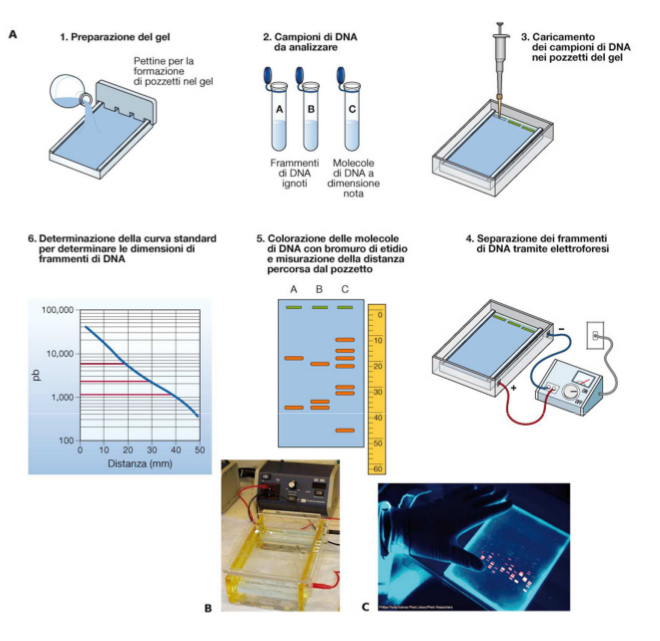
\includegraphics[scale=1.00]{img/66_Elettroforesi.png}
\caption{}
\label{elettroforesi}
\end{figure}

Per poter visualizzare lo spostamento dei frammenti di DNA su un gel,
altrimenti invisibili, è necessario applicare un colorante specifico
come il \emph{bromuro di etidio} (mutageno). Questa sostanza si
intercala tra i due filamenti di DNA ed emette una fluorescenza di
colore arancione quando esposta a raggi UV.

\begin{figure}[htp]
\centering
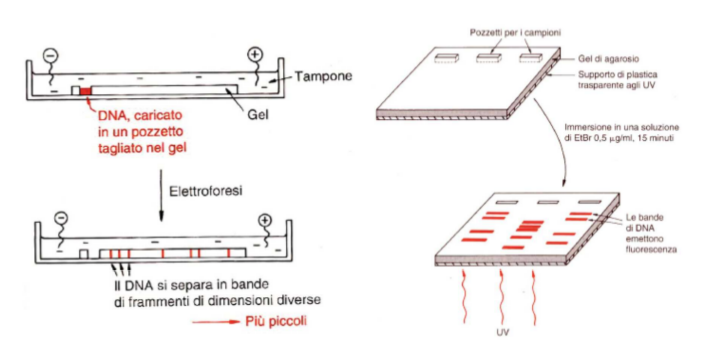
\includegraphics[scale=1.00]{img/64_Elettroforesi su gel.png}
\caption{}
\label{elettroforesi-su-gel}
\end{figure}

Il DNA sottoposto ad un campo elettrico migra ad una \emph{velocità
proporzionale all'inverso del log 10 del suo peso molecolare}.

\textbf{D = a-b(LogM)}

Dove:

\begin{itemize}
\itemsep1pt\parskip0pt\parsep0pt
\item
  \textbf{D} è la distanza coperta;
\item
  \textbf{M} è il peso molecolare del frammento;
\item
  \textbf{a} e \textbf{b} sono costanti.
\end{itemize}

Facendo migrare il campione in esame insieme ad uno standard di
frammenti con pesi molecolari di dimensione nota è possibile estrapolare
il peso molecolare del campione ignoto.

Utilizzando questa serie di frammenti di DNA a peso molecolare noto è
possibile costruire una \textbf{curva di taratura}, dove ogni banda sul
gel corrisponde ad un punto le cui coordinate sono costituite, in
\textbf{ascissa}, dalla \textbf{distanza in cm dal pozzetto} e in
\textbf{ordinata}, dal \textbf{Log 10 del peso molecolare}. Congiungendo
tutti i punti, riportati su un grafico semi-logarittimico, si dovrebbe
formare una linea approssimativamente retta,da cui, nota la distanza dal
pozzetto percorsa da una banda incognita, è possibile estrapolare il
peso molecolare approssimativo.

\begin{figure}[htp]
\centering
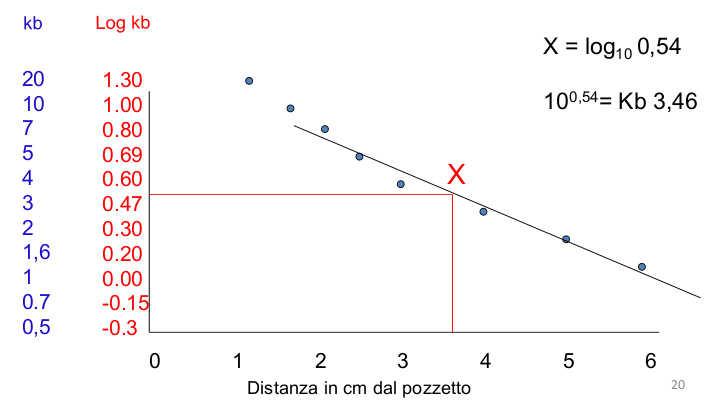
\includegraphics[scale=1.00]{img/65_Grafico peso molecolare elettroforesi.png}
\caption{}
\label{grafico-peso-molecolare-elettroforesi}
\end{figure}

\section{RNA interference}\label{rna-interference}

L'RNA interference consiste nel processo biologico in cui molecole di
RNA inibiscono l'espressione di un gene (solitamente causando la
distruzione di specifiche molecole di mRNA).

Storicamente questo fenomeno è stato indicato anche con altri nomi,
quali:

\begin{itemize}
\itemsep1pt\parskip0pt\parsep0pt
\item
  \textbf{co-soppressione}. Il fenomeno dell'interferenza è stato per
  prima scoperto nei vegetali. Nel 1990, Jorgenson e colleghi, cercando
  di ottenere un fiore di colore scuro, avevano introdotto un
  \textbf{transgene} per la \emph{chalone synthase} (responsabile della
  sintesi del pigmento anthocyanina) in cellule di petunia.
  Sorprendetemente, ottennero un fiore variegato. L'analisi delle
  cellule bianche rivelò che in queste erano assenti i mRNAs sia del
  transgene che del gene endogeno Con co-soppressione (1990) si indica
  il fenomeno per cui l'introduzione di un gene esogeno codificante per
  l'\emph{enzima calcone sintasi} in petunia, silenzia sia il gene
  esogeno che quello endogeno;
\item
  un altro esempio di RNA interference è il \textbf{post-transcriptional
  gene silencing (PTGS)} del \emph{gene par-1} di C. elegans tramite
  l'introduzione di RNA antisenso. Lo stesso risultato venne ottenuto
  mediante l'introduzione di RNA senso usato come controllo negativo;
\item
  un altro fenomeno simile al PTGS è il \textbf{quelling}. Questo
  fenomeno è stato osservato in petunia ma avvenuto in una coltura di N.
  crassa trasformata con un plasmide contenente il \emph{gene al1}.
\end{itemize}

Nel 1998 gli studiosi Fire e Mello catalogarono tutti questi fenomeni
isolati sotto un principio comune: RNA interference (\textbf{RNAi}).

Continuando gli studi su C. elegans di Guo \& Kemphues per cercare delle
spiegazioni agli eventi da essi osservati, Fire e Mello ipotizzarono che
le preparazioni di RNA antisenso contenessero piccole quantità di RNA
senso e che la formazione di molecole ibride a doppio filamento
(\textbf{dsRNA}) fosse responsabile del silenziamento genico osservato
con l'anti-senso (RNAi).

I meccanismi responsabili del fenomeno possono essere:

\begin{itemize}
\itemsep1pt\parskip0pt\parsep0pt
\item
  il silenziamento trascrizionale del gene;
\item
  il silenziamento post-trascrizionale del gene (PTGS), l'mRNA è
  sintetizzato e poi degradato.
\end{itemize}

Nel 1995 Guo \& Kemphues, per dimostrare che avevano clonato il gene
par-1 (un gene necessario per la divisione mitotica dello zigote) di
C.elegans, condussero esperimenti di PTGS con oligonucleotidi antisenso.

Nel 1998, Fire \& Mello circonstanziarono che l'iniezione di dsRNA era
un modo molto efficiente per ottenere fenotipi mutanti in C.elegans.

L'introduzione di una soluzione contenente filamenti di RNA senso ed
antisenso era almeno dieci volte più efficace dei filamenti singoli.

Le analisi elettroforetiche mostrarono che, all'interno dell'organismo,
il materiale iniettato si conformava per la maggior parte come doppio
filamento (dsRNA, RNA double strand) infatti le molecole di ssRNA
(single strand RNA) venivano rapidamente degradate nel citoplasma.

Di contro, osservarono che un tempo prolungato tra l'iniezione del
filamento senso e di quello antisenso dava un calo drastico
dell'efficienza fino alla totale assenza di effetto.

Sorprendentemente, gli effetti di questa interferenza genica si
mostravano sia nei soggetti iniettati che nella progenie.

Che cos'è la RNA interference? Un fenomeno in cui l'espressione (o
introduzione) di un RNA a doppio filamento (dsRNA) in un diverso range
di organismi e tipi cellulari causa la degradazione di un mRNA bersaglio
complementare.

\section{Formazione e azione di siRNA e
miRNA}\label{formazione-e-azione-di-sirna-e-mirna}

\subsection{Biochimica dei siRNA (small interfering
RNA)}\label{biochimica-dei-sirna-small-interfering-rna}

\textbf{Fase iniziatrice}: Dicer processa lunghe molecole di dsRNA in
siRNA maturi di 21-23 bp con 2 nt liberi e complementari al 3' e un
monofosfato al 5'.

\textbf{Fase effettrice}: siRNA viene incorporato nel RISC che lo
denatura. Il filamento antisenso giuda il legame del RISC all'mRNA
bersaglio causandone la degradazione.

Possibili applicazioni degli siRNA sono:

\begin{itemize}
\itemsep1pt\parskip0pt\parsep0pt
\item
  determine la funzione di un gene;
\item
  studiare ``persorsi biologici'' (pathways)
\item
  identificare e convalidare bersagli;
\item
  generare modelli knock-out.
\end{itemize}

Nel futuro gli siRNA potranno essere utilizzati per terapie mediche.

Esistono almeno 5 modi per produrre gli siRNA:

\begin{enumerate}
\def\labelenumi{\arabic{enumi}.}
\itemsep1pt\parskip0pt\parsep0pt
\item
  tramite sintesi chimisa;
\item
  tramite trascrizione in vitro;
\item
  tramite digestione di lunghi dsRNA da parte di un enzima della
  pamiglia delle RNA polimerasi III;
\item
  tramite l'espressione in cellule da un siRNA plasmidiale o un vettore
  virale (?);
\item
  tramite l'espressione in cellule da un siRNA derivato da PCR (??).
\end{enumerate}

Nel disegno di un siRNA funzionale vi sono parametri di basi che devono
essere considerati:

\begin{itemize}
\itemsep1pt\parskip0pt\parsep0pt
\item
  la regione target deve essere \emph{a valle del codone di inizio}
  della traduzione, ad una distanza che varia dalle 50 alle 100bp;
\item
  l'mRNA target deve avere dal 5' al 3' una sequenza AA(N19)UU;
\item
  l'mRNA target deve avere un contenuto in GC del 30-70\%;
\item
  devono essere evitate le regioni UTR (untraslated region) sia al 3'
  che al 5';
\item
  il filamento antisenso deve essere termodinamicamente instabile al 5'
  rispetto al 3', favorendone l'incorporazione nel RISC;
\item
  devono essere evitate regioni polimorfiche tranne nel silenziamento
  allele-specifico;
\item
  devono essere evitati più di 3 mismatch rispetto al target.
\end{itemize}

\subsection{Biogenesi dei miRNA}\label{biogenesi-dei-mirna}

Alcuni miRNA derivano da sequenze non codificanti, altri sono contenuti
all'interno di regioni introniche di sequenze codificanti spesso nello
stesso senso, suggerendo una possibile trascrizione insieme al gene
ospite.

I miRNA vengono inizialmente trascritti dall'\emph{RNA polimerasi II} a
partire dal loro stesso promotore a \textbf{pri-miRNA (primary miRNA)}

I pri-miRNA sono sequenze a singolo filamento con struttura secondaria a
forcina, e complementarietà interna alla sequenza non perfetta. I
pri-miRNA vengono processati da parte di una ribonucleasi di classe III
(RNAsi III), chiamata \textbf{Drosha}, in \textbf{pre-miRNA (precursor
mi-RNA)}. I pre-miRNA sono sequenze a singolo filamento lunghe circa 70
nt, con una struttura secondaria a forcina e una complementarietà
interna non perfetta.

I pre-miRNA vengono trasportati dal nucleo al citoplasma attraverso
l'\textbf{Esportina 5} in cooperazione con \textbf{Ran-GTP}.

Nel citoplasma, ad opera di Dicer, i pre-miRNA vengono tagliati a miRNA
maturi. Questi sono formati da sequenze di dsRNA lunghe circa 21-25 nt,
prive della struttura a forcina che viene tagliata da Dicer. Questo
taglio lascia 2 nt simmetrici liberi al 3' ed un monofosfato al 5' della
stessa terminazione.


\begin{figure}[htp]
\centering
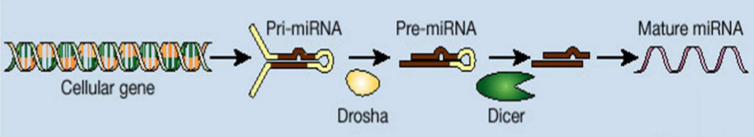
\includegraphics[scale=1.00]{img/67_miRNA.png}
\caption{}
\label{mirna}
\end{figure}

\subsection{Gli RNAi}\label{gli-rnai}

RNAi sono conservati tra le specie.

Le funzioni biologiche degli RNAi sono diverse, tra cui:

\begin{itemize}
\itemsep1pt\parskip0pt\parsep0pt
\item
  \emph{regolazione dell'espressione genica} (tempi di sviluppo,
  specificità del tessuto, adattamento);
\item
  \emph{difesa da patogeni} quali i virus a dsRNA.
\end{itemize}

Come possiamo utilizzare queste conoscenze per studiare i meccanismi
delle malattie e curarle?

Gli RNAi possono essere utilizzati per diversi scopi:

\begin{itemize}
\itemsep1pt\parskip0pt\parsep0pt
\item
  per \textbf{indurre la sovraespressione di un determinato gene}.
  Questo meccanismo viene detto \textbf{``gain of function''} ed è un
  metodo efficace con cui identificare i geni che influenzano lo
  sviluppo di particolari strutture o tipi di cellule. Il gain of
  function induce un incremento dell'espressione del gene bersaglio, o
  un espressione ``de novo'' del gene, influendo sul fenotipo cellulare;
\item
  per \textbf{inserire nuovi geni} nel DNA ospite. La differenza tra
  organismi \textbf{knock-in} e organismi transgenici, è che nel
  knock-in il gene estraneo è inserito in un locus specifico nel genoma
  bersaglio tramite ricombinazione omologa. Negli organismi transgenici
  invece, il gene che si desidera integrare può finire ovunque nel
  genoma dell'organismo ospite;
\item
  per \textbf{identificare il ruolo di un determinato gene} attraverso
  il suo spegnimento tramite \textbf{``loss of function''}. La RNAi
  permette di svolgere studi di loss of function \emph{senza eliminare
  fisicamente un gene} tramite un processo di **``knock-down\textbf{. Il
  processo di eliminazione fisica di un gene per impedirne l'espressione
  viene definito }knock-out**. I vantaggi di questa modalità consistono
  tra l'altro nella possibilità di ripristinare l'attività del gene
  silenziato attraverso l'utilizzo di sistemi di transgenesi
  condizionale.
\end{itemize}

Le possibili molecole sintetizzabili in vitro sono:

\begin{itemize}
\itemsep1pt\parskip0pt\parsep0pt
\item
  \textbf{siRNA} che una volta introdotti non vengono processati da
  Dicer e vengono direttamente incorporati nel RISC;
\item
  \textbf{lunghe molecole di dsRNA} che invece devono essere processate
  da Dicer;
\item
  \textbf{short hairpin RNA (shRNA)}, molecole di RNA di 50-70 nt che
  formano una struttura a forcina con perfetta complementarietà dei
  bracci e che tagliati da Dicer generano siRNA funzionali;
\item
  \textbf{miRNA-based hairpin RNA}, duplex di RNA a forcina con una non
  perfetta complementarietà tra i bracci. Emulano i pre-miRNA che
  fuoriescono dal nucleo e una volta processati da Dicer generaro i
  miRNA;
\end{itemize}

\subsubsection{Produzione di shRNA}\label{produzione-di-shrna}

Esistono diversi metodi per la produzione di shRNA:

\begin{itemize}
\itemsep1pt\parskip0pt\parsep0pt
\item
  \textbf{sintesi chimica di oligonucleotidi} di 50-70 nt, appaiati e
  ligati in un vettore. È un metodo relativamente semplice, anche se la
  sintesi di un oligonucleotide così lungo è più soggetta ad errori;
\item
  \textbf{trascrizione ad opera dell'RNA polimerasi III} a partire da un
  unico promotore (U6 o H1), di sequenze invertite codificanti per uno
  shRNA a forcina. Questo sarà poi processato da Dicer, i cui tagli
  genereranno siRNA funzionali per complessi RISC.
\end{itemize}

\subsubsection{RNAi in cellule di
mammifero}\label{rnai-in-cellule-di-mammifero}

Nei mammiferi si riscontrano molte più difficoltà nell'indurre l'RNAi
perché, a seguito dell'introduzione di una molecola di dsRNA, si ha
l'attivazione di un sistema di \textbf{inibizione totale
dell'espressione}, piuttosto che di un sistema sequenza-specifico.
Questo avviene poichè interagisce con le molecole di dsRNA una proteina
kinasica (PKR) che scatena la risposta immunitaria dell'interferone,
bloccando globalmente la trascrizione. Utilizzando i siRNA, invece, si è
riusciti ad indurre il silenziamento sequenza-specifico, senza scatenare
la risposta interferonica. Questa scoperta è molto utile al fine di
poter progettare metodologie di somministrazione umana a scopo
terapeutico.

In linea di principio, qualunque malattia causata dall'espressione di
forme aberranti di un gene (es. mutazioni), o dall'aumento
dell'espressione di una o di un numero limitato di proteine, può essere
trattata mediante \textbf{RNAi therapy}. Anche patologie parassitarie
(virus, batteri, protozoi) rappresentano un potenziale bersaglio
terapeutico.

\begin{figure}[htp]
\centering
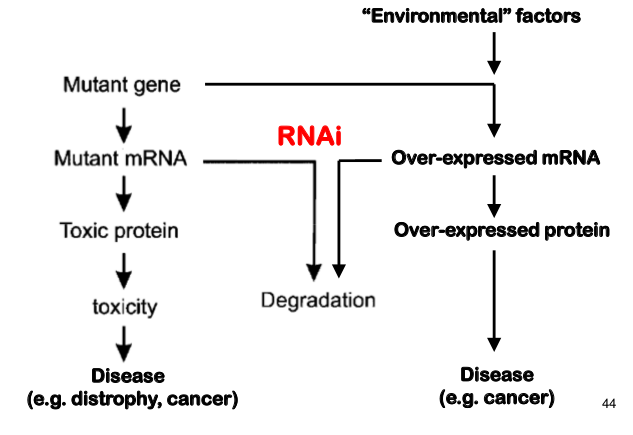
\includegraphics[scale=1.00]{img/68_miRNA-therapy.png}
\caption{}
\label{mirna-therapy}
\end{figure}

I vantaggi principali degli RNAi sulle piccole molecole e proteine
terapeutiche sono che tutti i bersagli, inclusi quelli che rispondo e
non rispondono ai farmaci, extracellulari e intracellulari e alleli
mutanti possono essere ``mirati'' con gli RNAi. Uno dei maggiori
vantaggi delle tecnologie basate sul riconoscimento di sequenze è la
possibilità di produrre farmaci precisamente ``disegnati'' per quasi
ogni sequenza bersaglio (sia codificante che non codificante),
indifferentemente dalla funzione del prodotto genico.

\subsubsection{Terapia basata sui siRNA}\label{terapia-basata-sui-sirna}

Lo scopo della terapia basata sui siRNA è quello di \textbf{attivare la
degradazione} di un selettivo mRNA per un efficiente silenziamento
genico. La terapia con RNAi offre potenzialmente diversi vantaggi:
quali:

\begin{itemize}
\itemsep1pt\parskip0pt\parsep0pt
\item
  una diffusa applicabilità;
\item
  precisione terapeutica;
\item
  selettività;
\item
  assenza di effetti indesiderati;
\item
  relativa facilità di produzione;
\item
  bassi costi di produzione.
\end{itemize}

Possibili malattie alle quali potrebbe essere applicata la siRNA therapy
sono: infezioni virali, cancro, malattie metaboliche, malattie
genetiche, ecc\ldots{}

È possibile raggiungere il pathway endogeno attraverso 2 vie:

\begin{itemize}
\itemsep1pt\parskip0pt\parsep0pt
\item
  tramite un \emph{vettore virale} per esprimere shRNA;
\item
  tramite un \emph{siRNA che mimi il prodotto di clivaggio di Dicer nel
  citoplasma} incorporandosi direttamente nel complesso RISC.
\end{itemize}

I siRNA sono più attraenti dal punto di vista terapeutico perchè entrano
nel pathway dell'RNAi in modo consistente e prevedibile, e non
interferiscono con la regolazione genica da parte dei miRNA endogeni.
Per tali motivi i siRNA sono più avanzati negli studi clinici e
preclinici della terapia con RNAi.

\paragraph{Selezione in vitro}\label{selezione-in-vitro}

Ci sono diversi step nell'identificazione di possibili siRNA candidati:

\begin{itemize}
\itemsep1pt\parskip0pt\parsep0pt
\item
  un \emph{disegno bioinformatico};
\item
  \textbf{studi in vitro} per determinare:

  \begin{enumerate}
  \def\labelenumi{\arabic{enumi}.}
  \itemsep1pt\parskip0pt\parsep0pt
  \item
    l'\emph{efficacia di silenziamento};
  \item
    l'\emph{assenza di effetti indesiderati};
  \item
    l'introduzione di eventuali modificazioni chimiche per aumentare
    \textbf{stabilità} e \textbf{specificità}
  \end{enumerate}
\item
  \emph{selezione delle tecniche} più adatte \emph{per il trasferimento}
  in cellule/tessuti/organismi specifici da trattare.
\end{itemize}

Le 3 principali caratteristiche da tenere in considerzione nel disegno e
nella selezione di un siRNA candidato sono:

\begin{itemize}
\itemsep1pt\parskip0pt\parsep0pt
\item
  \textbf{potenza};
\item
  \textbf{speicficità};
\item
  \textbf{stabilità}.
\end{itemize}

Sono da evitare o minimizzare 2 tipi di effetti:

\begin{itemize}
\itemsep1pt\parskip0pt\parsep0pt
\item
  il silenziamento di geni che mostrano omologia parziale con il siRNA;
\item
  lo sviluppo di una risposta immunitaria.
\end{itemize}

Oggi è possibile selezionare nell'arco di poche settimane/mesi siRNA
candidati potenti, stabili e specifici in vitro e con effetti
indesiderati mitigati.

La \textbf{potenza}. Un siRNA candidato nel silenziamento di un gene
target è \emph{potente} quando la sua attività si esplica a
\textbf{basse concentrazioni} (solitamente nanomolari). siRNA potenti
possono essere identificati mediante l'uso di algoritmi, o valutando
tutte le possibili sequenze generabili da un mRNA, per poi selezionare
quelle che inducono silenziamento efficiente a concentrazioni più basse.
Sono più potenti siRNA di 27nt rispetto a 19nt ma sono più difficili da
sintetizzare e hanno maggiore probabilità di attivare una risposta
immunitaria.

La \textbf{specificità}. Un siRNA è \emph{specifico} quando è in grado
di indurre il \textbf{silenziamento solo di uno specifico mRNA}.
Esistono 2 problemi che limitano la specificità di un siRNA:

\begin{enumerate}
\def\labelenumi{\arabic{enumi}.}
\itemsep1pt\parskip0pt\parsep0pt
\item
  il riconoscimento e, quindi, \textbf{silenziamento di mRNA con
  omologia parziale};
\item
  lo sviluppo della \textbf{risposta immunitaria} per \emph{attivazione
  della PKR}, ad opera di molecole di dsRNA lunghi più di 30nt, e per
  \emph{attivazione del TLR (toll-like receptor)}, espresso sulle
  cellule dendritiche, con conseguente produzione di interferone e di
  citochine pro-infiammatorie. Sembra che le isole CpG del filamento
  antisenso attivino il TLR.
\end{enumerate}

Il problema del silenziamento di mRNA con omologia parziale può essere
minimizzato attraverso:

\begin{itemize}
\itemsep1pt\parskip0pt\parsep0pt
\item
  un \textbf{disegno attento dei siRNA};
\item
  una \textbf{modificazione chimica dei ribosi} nel filamento guida, e
  in particolare attraverso l'aggiunta di un gruppo metilico al gruppo
  OH in 2' del nt 2 (2'-O-Met).
\end{itemize}

La \textbf{stabilità}. Gli siRNA sono normalmente degradati nel plasma
umano con un'emivita di pochi minuti. Per \textbf{aumentare l'emivita} e
quindi la \emph{stabilità} dei siRNA, si introducono diverse
modificazioni chimiche: + l'aggiunta di un fosforotioato (P=S) al 3'
protegge dalla digestione da parte delle esonucleasi; + l'aggiunta del
gruppo metile o di un atomo di Fluoro al 2' del ribosio (2'-O-Met o
2'-F) protegge dalla digestioni dalle endonucleasi.

Queste modificazioni sono necessarie perché è importante che i siRNA
raggiungano intatti i tessuti bersaglio.

Un'altra considerazione importante nel disegnare un siRNA a scopi
terapeutici è trovare, se possibile, un target conservato tra le specie
più usate per gli studi di efficacia e sicurezza, per costruire un solo
farmaco candidato da usare dalle fasi di ricerca di base fino agli studi
clinici. Perciò, l'approccio più prudente da seguire è quello di
identificare diverse molecole candidate adatte a studi in vivo per poi
selezionare quelle più potenti, specifiche, stabili e con minore
attività immuno-stimolatoria.

\paragraph{Vie di somministrazione in
vivo}\label{vie-di-somministrazione-in-vivo}

Oggi esistono diverse metodologie di trasporto dei siRNA in vivo quali:

\begin{itemize}
\itemsep1pt\parskip0pt\parsep0pt
\item
  naked siRNA;
\item
  coniugati;
\item
  liposomi/lipoplesso;
\item
  complessi con peptidi/proteine;
\item
  complessi con anticorpi
\end{itemize}

La sfida principale riguarda lo sviluppo di tecnologie di trasporto
direttamente nella cellula/tessuto bersaglio per diminuire la dose di
efficacia richiesta, e diminuire gli effetti tossici e indesiderati
legati ad una somministrazione sistemica.

I \textbf{naked siRNA}. Consistono in una somministrazione di siRNA
(modificato o meno) in soluzione salina o in eccipienti semplici come il
destrosio 5\% (D5W).

La semplicità di formulazione e somministrazione direttamente nel
tessuto bersaglio rende questa via l'approccio terapeutico più
attrattivo.

I naked siRNA possono essere somministrati in diverse zone:

\begin{itemize}
\itemsep1pt\parskip0pt\parsep0pt
\item
  \textbf{nell'occhio}. L'iniezione intravitreale L'iniezione
  intravitreale di naked siRNA in soluzione salina vs VEGF rallenta la
  neovasvolarizzazione oculare in modelli animali di AMD (age-related
  macular degeneration). • L'iniezione intravitreale di naked siRNA in
  soluzione salina vs VEGFR1 riduce l'area di vascolarizzazione oculare
  nello stesso modello animale. • Partono clinical trials per testare
  siRNA vs VEGF in pazienti affetti da AMD.di naked siRNA in soluzione
  salina \textbf{vs VEGF} \emph{rallenta la neovascolarizzazione
  oculare} in modelli animali di AMD (age-related macular degeneration).
\end{itemize}

L'iniezione intravitreale di naked siRNA in soluzione salina \textbf{vs
VEGFR1} \emph{riduce larea di vascolarizzazione oculare} nello stesso
modello animale.

Partono clinical trials per testare siRNA vs VEGF in pazienti affetti da
AMD;

\begin{itemize}
\itemsep1pt\parskip0pt\parsep0pt
\item
  \textbf{nel polmone}. L'instillazione intranasale di naked siRNA in
  soluzione salina \textbf{vs geni di RSV (respiratory syncytial virus)}
  e del \textbf{virus della parainfluenza}, due delle principali cause
  di ospedalizzazione pediatrica negli USA oggi, ne riduce lo sviluppo e
  quindi i sintomi patologici quali: produzione di leucotrieni,
  infiammazione polmonare e stress respiratorio.
\end{itemize}

La somministrazione intranasale di naked \textbf{siRNA in D5W vs i geni
del CoronaVirus in modelli animali di SARS (severe acute respiratory
syndrome)}, ne inibisce la replicazione virale e ne riduce gli effetti
patologici.

La somministrazione intranasale di naked siRNA \textbf{vs la
eme-ossigenasi1 (HMOX1)}, risulta in un aumento dell'apoptosi dopo
riperfusione a seguito di ischemia, dimostrando che in questo caso
l'induzione di tale gene è \textbf{protettivo};

\begin{itemize}
\itemsep1pt\parskip0pt\parsep0pt
\item
  \textbf{nel SNC}. La somministrazione di naked siRNA in soluzione
  salina intracerebrovascolare, intratecale o intraparenchimale, causa
  il silenziamento di specifici mRNA target neuronali in più regioni del
  SNC e periferico. Poiché è richiesta una dose maggiore e poiché
  l'assunzione dei siRNA non è omogenea, sembra essere favorita la
  somministrazione di coniugati lipidici.
\end{itemize}

Gli \textbf{siRNA coniugati}. Consistono nella coniugazione covalente
dei siRNA a molecole bersaglio quali:

\begin{itemize}
\itemsep1pt\parskip0pt\parsep0pt
\item
  molecole lipofile;
\item
  proteine;
\item
  peptidi;
\item
  aptameri.
\end{itemize}

Le molecole vengono, generalmente, coniugate al 5' o al 3' del filamento
senso senza distruggere l'attività di quello antisenso.

\begin{itemize}
\itemsep1pt\parskip0pt\parsep0pt
\item
  \textbf{Coniugazione con colesterolo}.
\end{itemize}

L'iniezione intravena di \textbf{siRNA vs l'APOB} il cui filamento senso
è coniugato al 5' con una molecola di colesterolo, causa una riduzione
del suo mRNA nel fegato e nel digiuno, una riduzione della proteina nel
plasma e, quindi, una riduzione del colesterolo sierico.

\begin{itemize}
\itemsep1pt\parskip0pt\parsep0pt
\item
  \textbf{Coniugazione con liposomi e lipoplessi}.
\end{itemize}

I \textbf{liposomi} sono vescicole costituite da un compartimento
acquoso racchiuso in un doppio strato fosfolipidico che, fondendosi con
la membrana delle cellule, permette il trasporto in esse del materiale
contenuto nel compartimento acquoso.

Farmaci polari possono essere incorporati nel compartimento acquoso ed
essere, quindi, veicolati nelle cellule tramite i liposomi. In questo
modo si migliorano le caratteristiche farmaco-cinetiche del farmaco e se
ne riduce la tossicità.

I \textbf{lipolessi} sono costituiti da lipidi che complessano con gli
acidi nucleici a formare particelle amorfe: solitamente si formano
miscelando siRNA con alcuni agenti di trasfezione come la lipofectamina
e il transit-TKO.

Sia i liposomi che i lipoplessi sono molto usati, sia in vivo che in
vitro, per il trasferimento di siRNA. Sono stati descritti diversi
successi sia di somministrazione locale che sistemica con entrambi.

La \textbf{somministrazione sistemica} consiste in una
\emph{somministrazione intravena di lipoplessi} con \textbf{siRNA vs
l'APOB (apolipotroteina B)} ne riduce notevolmente i livelli di mRNA e,
quindi, di colesterolo, sia in modelli murini che in primati non umani.

La somministrazione intravena di lipoplessi cationici contenenti
\textbf{siRNA vs il TNF}, ne riducono la produzione a livello delle
giunture del ginocchio in modelli animali di artrite remautoide.

La somministrazione intravena di liposomi contenenti \textbf{siRNA vs la
CAVEOLINA-1} ne riduce l'espressione di circa il 90\% nell'endotelio
polmonare di topo e risulta, quindi, in un aumento della permeabilità
vascolare.

La \textbf{somministrazione locale} consiste nella
\emph{somministrazione subretinale di lipoplessi} in Transit-TKO con
\textbf{siRNA vs VEGF}, riduce la neovascolarizzazione coroidale in
modelli animali di AMD.

La somministrazione subcongiuntivale di lipoplessi in Transit-TKO con
\textbf{siRNA vs TGF\(\beta\)R2}, sopprime l'infiammazione e la fibrosi
oculare in modelli animali.

L'\emph{iniezione intracranica} di liposomi contenenti \textbf{siRNA vs
geni virali}, protegge il topo dal virus dell'encefalite giapponese.

L'\emph{iniezione intratumorale} di lipoplessi con \textbf{siRNA vs i
geni E6-E7 del PV} causa una inibizione della crescita tumorale e la
soppressione dell'espressione dei geni virali.

\begin{itemize}
\itemsep1pt\parskip0pt\parsep0pt
\item
  \textbf{Coniugazione con peptidi/polimeri}
\end{itemize}

I siRNA possono essere complessati con peptidi e polimeri cationici
attraverso interazioni ioniche con i loro fosfati carichi negativamente,
a formare nanoparticelle stabili.

Importante è prevenire l'aggregazione e controllare le dimensioni delle
particelle, solitamente tramite l'incorporazione di molecole come il PEG
(polietilen glicole) che le stabilizzano e ne migliorano le proprietà
farmacocinetiche.

All'interno di queste particelle possono essere introdotte altre
molecole quali \emph{trasferrina}, \emph{folati}, \emph{mannosio},
\emph{galattosio}, \emph{peptide RGD (Arg-Gly-Asp)} che migliorano e
accelerano la specificità di trasporto del siRNA solo vs le cellule che
ne esprimono i recettori.

Un polimero che si può complessare ai siRNA è il \textbf{PEI
(polietilen-immina)}. Questo è un polimero sintetico, lineare o
ramificato, con elevata densità di cariche cationiche. Il PEI
interagisce elettrostaticamente con la superficie delle cellule, viene
poi endocitato e, infine, disgrega gli endosomi in quanto causa un
aumento del flusso protonico e di acqua che li disgrega, permettendo
così il rilascio del siRNA nel citoplasma.

Complessi con PEI di siRNA vs pleiotropina, VEGF e HER2 (human epidermal
growth factor receptor 2) hanno attività antitumorale. Lo svantaggio
risiede nell'estrema tossicità associata ad elevate dosi di PEI.

Residui di istidina e poli lisina sembrano avere efficacia in vitro
simile al PEI.

\begin{itemize}
\itemsep1pt\parskip0pt\parsep0pt
\item
  \textbf{Complessi con anticorpi}
\end{itemize}

Gli anticorpi possono essere usati per trasportare siRNA in specifiche
cellule bersaglio.

\paragraph{Clinical trials}\label{clinical-trials}

Ci sono 3 clinical trials in fase di studio:

\begin{enumerate}
\def\labelenumi{\arabic{enumi}.}
\item
  \textbf{siRNA CAND5 vs tutte le isoforme del VEGF-A} ha completato la
  fase 2 dei clinical trials in pazienti con una forma progressiva grave
  di AMD. Vantaggi:

  \begin{itemize}
  \itemsep1pt\parskip0pt\parsep0pt
  \item
    facilità di somministrazione direttamente sul tessuto bersaglio;
  \item
    ambiente oculare relativamente libero da nucleasi;
  \end{itemize}
\item
  \textbf{siRNA 0-27 vs il VEGFR1} ha completato la fase 1 in assenza di
  tossicità in pazienti affetti da edema maculare diabetico;
\item
  \textbf{siRNA ALN-RSV01 vs il gene del nucleocapside di RSV} ha
  completato la fase 1 in assenza di tossicità in 100 volontari sani.
  Vantaggi:

  \begin{itemize}
  \itemsep1pt\parskip0pt\parsep0pt
  \item
    facilità di trasporto direttamente nel tessuto bersaglio (cellule
    endoteliali polmonari);
  \item
    ambiente polmonare relativamente povero di nucleasi;
  \item
    la somministrazione per inalazione non è invasiva;
  \item
    assenza di metabolismo di primo passaggio che comporta la riduzione
    della dose necessaria e degli effetti avversi sistemici.
  \end{itemize}
\end{enumerate}

La sfida principale nell'usare RNAi a scopi terapeutici rimane quella di
superare una serie di barriere che limitano l'efficienza di trasporto
dei siRNA all'interno delle cellule/tessuti bersaglio, quali:

\begin{itemize}
\itemsep1pt\parskip0pt\parsep0pt
\item
  il raggiungimento delle adeguate proprietà farmacocinetiche per
  aumentare l'esposizione del farmaco alle cellule bersaglio;
\item
  il raggiungimento di meccanismi che promuovano l'assunzione cellulare
  e il rilascio del farmaco nel citoplasma;
\item
  l'instabilità nel siero;
\item
  l'eliminazione tramite le urine;
\item
  la distribuzione non specifica.
\end{itemize}

È inoltre, necessaria l'introduzione di \textbf{sistemi REPORTER} sia
esogeni che endogeni per identificare l'effettivo trasporto del farmaco
all'interno delle cellule. È fondamentale, infine, rispettare i
parametri di efficacia e sicurezza.

I limiti nell'utilizzo di terapie basate sull'RNA interference sono:

\begin{itemize}
\itemsep1pt\parskip0pt\parsep0pt
\item
  gli elevati dosaggi richiesti;
\item
  la necessità di ripetere i trattamenti;
\item
  i costi dei farmaci a siRNA;
\item
  la stabilità nell'organismo;
\item
  gli effetti ``off-target'', ovvero il rischio di reprimere altri geni.
\end{itemize}

Gli RNAi ci permettono di investigare le funzioni dei vari geni
spegnendoli in maniera selettiva.

\end{document}
